\documentclass[10pt,twocolumn,letterpaper]{article}
\usepackage[review]{cvpr}
\usepackage{graphicx,booktabs,multirow,amsmath,amssymb,xcolor,enumitem,xspace}
\usepackage{microtype}
\usepackage{caption}
\captionsetup{font=small,labelfont=bf,skip=4pt}
\newcommand{\pithree}{$\pi^3$\xspace}
\newcommand{\vggt}{VGGT\xspace}
\newcommand{\auc}{AUC@3\xspace}
\newcommand{\aucc}{AUC@30\xspace}
\newcommand{\ci}[2]{[$#1$,\,$#2$]}
\usepackage{adjustbox}

\definecolor{cvprblue}{rgb}{0.21,0.49,0.74}
\usepackage[pagebackref,breaklinks,colorlinks,allcolors=cvprblue]{hyperref}
\usepackage[capitalize]{cleveref}
\crefname{section}{Sec.}{Secs.}
\Crefname{section}{Section}{Sections}
\crefname{table}{Tab.}{Tabs.}
\crefname{figure}{Fig.}{Figs.}

\def\paperID{*****}
\def\confName{CVPR}
\def\confYear{2027}

\title{Where Do Feed-Forward 3D Models Use Resolution?\\Probing VGGT and $\pi^3$}
\author{Anonymous CVPR submission\\\\Paper ID \paperID}

\begin{document}
\twocolumn[{%
\renewcommand\twocolumn[1][]{#1}%
\maketitle
\vspace{-1.6em}
\begin{center}
  \centering
  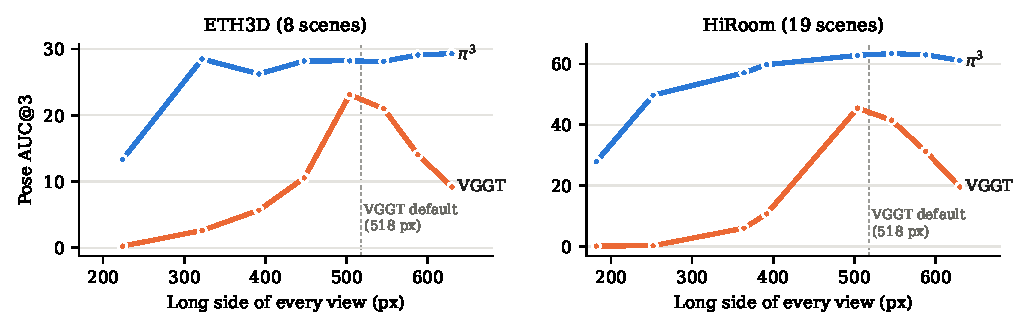
\includegraphics[width=\textwidth]{figures/fig_response.pdf}
  \captionof{figure}{\textbf{The two models respond to resolution in opposite ways.} Pose accuracy (\auc, higher is better) when all 12 views of a scene are resized to one size, from the smallest to the largest we tested. VGGT is best near the 518\,px width it uses by default and loses accuracy on both sides of it. \pithree improves with resolution and then levels off, with no significant decline in the tested range. Comparing the two models at a single size therefore gives very different answers depending on the size chosen.}
  \label{fig:response}
\end{center}
\vspace{0.8em}
}]
\begin{abstract}
Feed-forward 3D models such as VGGT and \pithree estimate cameras and geometry from a set of images in one forward pass, and their cost grows with the number of image tokens they process. Yet it is not clear how they use resolution: how their accuracy changes when the input is made larger or smaller, and which parts of the network actually need full resolution. We study these questions with frozen models and controlled probes. Each probe lowers the resolution at one stage of the network, such as the input pixels, the image encoder or global attention, for most of the views of a scene, and measures what is lost. We find that the two models respond to resolution in opposite ways: VGGT is accurate only near the input width it uses by default and degrades on both sides of it, while \pithree improves with resolution and then levels off. Resolution is not consumed at a single stage. For \pithree, lowering it in the encoder alone or in global attention alone costs most of what lowering it everywhere costs. Removing fine pixel detail while keeping the input size does not hurt \pithree, but it does hurt VGGT. In global attention, the views' queries need full resolution more than their keys. The models' errors at different input sizes are largely shared, so fusing predictions made at several sizes does not help. Finally, we show that 7-Scenes cannot resolve rotation differences below about 2\textdegree, which limits fine-grained comparisons on that benchmark.
\end{abstract}

\section{Introduction}
\label{sec:intro}

Feed-forward multi-view models now recover cameras and dense geometry from a set of unposed images in a single forward pass~\cite{wang2024dust3r,leroy2024mast3r,wang2025vggt,wang2025pi3}. VGGT~\cite{wang2025vggt} and \pithree~\cite{wang2025pi3} cut each view into $14{\times}14$ patches, encode them with a vision transformer, and then alternate attention within each view and across all views. Every patch is a token, so the resolution of the input decides how much the model costs to run. Resolution is also the main knob a practitioner can turn without retraining: images can be resized before they enter the model, and recent work changes how tokens are produced or kept inside it~\cite{goodtoken2026,redt2026,hdvggt2026}.

These choices rest on an assumption that is rarely tested: that more resolution helps, and that it helps everywhere in the network. If a model's accuracy saturates at some size, larger inputs only add cost. If one stage of the network can work at lower resolution without loss, that stage is where compute can be saved. If accuracy depends on a particular input size, comparisons between models at one size may say more about the size than about the models.

The goal of this paper is to measure how these models use resolution. We consider two properties. The first is the model's \emph{response} to resolution: how its accuracy changes when every view is made larger or smaller. The second is \emph{where} resolution is used: which stages of the network lose accuracy when their own resolution is lowered while the rest of the network keeps full resolution. We study both with frozen weights. For the second, we design probes that lower the resolution at a single stage, for 8 of the 12 views of a scene, while holding everything else fixed (\cref{tab:probes}). This lets us attribute a loss in accuracy to a stage rather than to the input as a whole.

Our experiments show the following.
\begin{itemize}[nosep,leftmargin=*]
  \item \textbf{The two models respond to resolution in opposite ways} (\cref{fig:response}). VGGT is most accurate near the 518\,px width it uses by default and loses much of its accuracy on either side of it. \pithree improves with resolution and then levels off. At one fixed size, VGGT can look nearly ten times worse than \pithree; at each model's best tested size, the gap is far smaller.
  \item \textbf{Resolution is needed at more than one stage.} For \pithree, lowering the encoder's resolution alone, or global attention's alone, costs most of what lowering it everywhere costs. Restoring full resolution in the encoder and frame attention while global attention stays low recovers only 2--30\% of the loss.
  \item \textbf{The models differ in whether they use fine pixel detail.} Removing detail above half resolution, while keeping the input size, does not hurt \pithree but costs VGGT 2.5 to 6 \auc.
  \item \textbf{In global attention, queries need resolution more than keys.} Pooling only the keys and values of the reduced views costs about 2 \auc; pooling their queries as well costs about twice as much.
  \item \textbf{Errors at different input sizes are correlated.} Fusing the poses predicted at two or three sizes never beats the best single size of no greater cost.
  \item \textbf{7-Scenes has a precision floor.} Three unrelated pose estimators, including classical two-view geometry, agree with its ground truth only to about 1.6--2.2\textdegree{} on well-matched pairs, so differences in \auc on this dataset should be read with care.
\end{itemize}

\section{Related work}
\label{sec:related}

\paragraph{Feed-forward multi-view reconstruction.}
DUSt3R~\cite{wang2024dust3r} and MASt3R~\cite{leroy2024mast3r} regress pointmaps for pairs of images and align them globally to handle more views. VGGT~\cite{wang2025vggt} processes all views jointly and predicts cameras, depth and points directly. \pithree~\cite{wang2025pi3} removes VGGT's reference view and makes the network equivariant to the order of its inputs. Depth Anything~3~\cite{lin2025da3} predicts depth and rays with a plain transformer and provides the benchmark data we use for ETH3D and HiRoom. These works report accuracy at one input resolution per model. We measure how accuracy changes across resolutions and inside the network.

\paragraph{Resolution and cost in these models.}
Several works reduce the cost of VGGT-style models. Good Token Hunting~\cite{goodtoken2026} restricts which frames each query attends to and spatially downsamples tokens within frames in selected layers, without training. ReDT~\cite{redt2026} trains a model that maps each view onto a fixed number of basis tokens, and HD-VGGT~\cite{hdvggt2026} trains a high-resolution branch on top of a low-resolution VGGT. These methods decide where tokens can be removed by designing or training a new procedure. Our probes ask the prior question of which stages of an existing model lose accuracy when their resolution is lowered.

\paragraph{Probing pretrained models.}
Probing studies measure what a frozen model represents by testing it under controlled conditions rather than by fine-tuning it. El Banani \etal~\cite{elbanani2024probing} probe the 3D awareness of visual foundation models this way. Vision transformers are also known to be sensitive to the resolution at which they are used: FlexiViT~\cite{beyer2023flexivit} and NaViT~\cite{dehghani2023navit} train models to cope with varying patch sizes and resolutions, and rotary position embeddings~\cite{su2024roformer}, which both of our models use, are commonly rescaled when the input length changes~\cite{chen2023pi,peng2023yarn}. We apply the probing approach to resolution in feed-forward 3D models.

\section{How a model uses resolution}
\label{sec:concept}

We first state what we mean by a model's use of resolution. A view of $h\times w$ pixels becomes $(h/14)(w/14)$ tokens, and every stage of the network then works on those tokens. Higher resolution gives the model finer image evidence and more tokens to compute with, at a higher cost. We posit that a model's use of resolution has two measurable aspects.

\paragraph{Response.} When every view of a scene is resized to the same size, accuracy should change smoothly with that size. A model that uses extra resolution well keeps improving until the images contain nothing more it can exploit, and then levels off. A model that has only learned to work at one size will peak at that size and degrade away from it, even when the larger input contains more information.

\paragraph{Stage use.} A feed-forward 3D model is a pipeline: pixels go into an image encoder, the encoder's tokens pass through frame attention (within each view) and global attention (across views), and prediction heads read the result. If a stage does not need full resolution, lowering its resolution while the rest of the network keeps it should cost nothing. If a stage does need it, the loss shows how much. Because the stages feed each other, the losses need not add up; a stage can be necessary without being sufficient.

These two aspects are not exhaustive, but they correspond to two practical questions: what input size to use, and where in the network compute can be saved.

\section{Experimental setup}
\label{sec:setup}

We aim to answer four questions:
\begin{enumerate}[nosep,leftmargin=*]
  \item How does accuracy change when every view is resized to one size?
  \item Which stages of the network need full resolution?
  \item Are the errors a model makes at different input sizes independent?
  \item How finely can the benchmark measure such differences?
\end{enumerate}

\paragraph{Models.}
We use the published weights of VGGT-1B~\cite{wang2025vggt} and \pithree~\cite{wang2025pi3} without fine-tuning. Both use $14{\times}14$ patches, a vision-transformer image encoder, and alternating frame and global attention with 2D rotary positions. VGGT treats its first view as a reference and uses a 518\,px input width by default; \pithree has no reference view. To run the probes, we reimplemented each model's forward pass as an explicit sequence of stages. Before every experiment, we verified in 32-bit precision that this decomposition reproduces the original model's outputs on real scenes (maximum absolute difference below $10^{-4}$). Experiments run in bfloat16 on a single GPU.

\begin{table}[t]
\centering\small
\setlength{\tabcolsep}{3pt}
\begin{adjustbox}{max width=\linewidth}
\begin{tabular}{@{}lcccc@{}}
\toprule
Probe & Pixels & Encoder & Frame att. & Global att. \\
\midrule
Full resolution        & full & full & full & full \\
Detail removed         & half$\uparrow$ & full & full & full \\
Encoder lowered        & half & half & full$^\dagger$ & full$^\dagger$ \\
Keys lowered           & full & full & full & keys half \\
Global lowered         & full & full & full & half$^\ddagger$ \\
All lowered            & half & half & half & half \\
\bottomrule
\end{tabular}
\end{adjustbox}
\caption{\textbf{Probes.} Each probe changes the resolution of one or more stages for 8 of the 12 views of a scene; the other 4 views stay at full resolution throughout. ``half$\uparrow$'': the image is reduced to half resolution and upsampled back, so the encoder receives a full-size image without its fine detail. $^\dagger$The encoder's half-resolution tokens are interpolated to the full grid. $^\ddagger$The views' tokens are pooled to half resolution before each global-attention block and the block's update is interpolated back; the prediction heads read these views at half resolution. All probes that use half-resolution positions map them onto the full-resolution grid.}
\label{tab:probes}
\end{table}

\begin{figure*}[t]
  \centering
  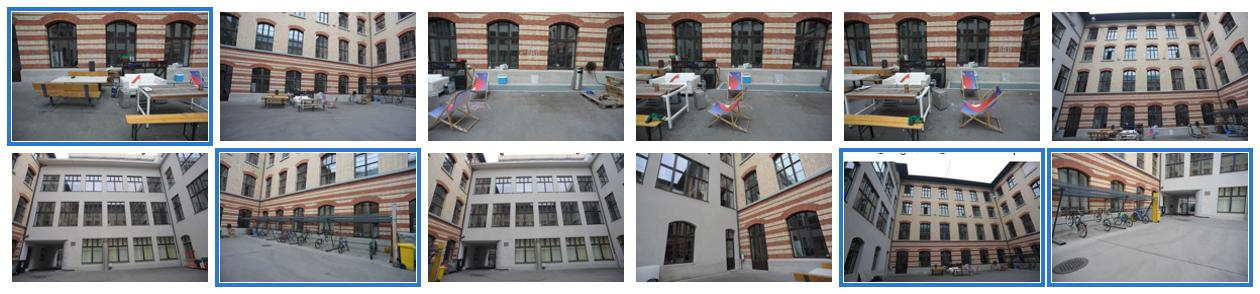
\includegraphics[width=\textwidth]{figures/fig_inputs.pdf}
  \caption{\textbf{The 12 input views of one ETH3D scene} (\emph{courtyard}), exactly as used in our ETH3D experiments, shown at reduced size. The 4 outlined views are the anchors, chosen by farthest-point sampling of the ground-truth camera centres; they stay at full resolution in every probe. The other 8 views are the ones whose processing each probe changes.}
  \label{fig:inputs}
\end{figure*}

\paragraph{Probes.}
Each scene gets 12 views. Four of them, chosen by farthest-point sampling of the ground-truth camera centres so that they spread over the scene, always stay at full resolution (\cref{fig:inputs}). These anchors give every probe the same full-resolution view of the scene's layout, so differences between probes come from how the other 8 views are processed. For the other 8 views, a probe lowers the resolution of specific stages by a factor of 2 per side (\cref{tab:probes}), which reduces their token count by about four and keeps every mapped position on an integer grid (\cref{eq:align}). \emph{Detail removed} keeps every stage at full resolution but feeds the encoder an image that has lost its fine detail; it measures whether the model uses pixel detail above half resolution. \emph{Encoder lowered} runs the encoder on the half-resolution image and interpolates its tokens to the full grid, so every later stage works at full resolution on coarser features. \emph{Keys lowered} keeps one query per full-resolution token in global attention but lets the other views read these 8 views only through keys and values area-pooled to the half-resolution grid; we add to the pooled keys' attention logits the logarithm of the number of full-resolution tokens each one replaces ($\log 3.83$ on 7-Scenes), so that a pooled key counts as the tokens it stands for. \emph{Global lowered} pools the queries as well. \emph{All lowered} runs every stage of these views at half resolution. Whenever a view's tokens sit on a half-resolution grid, we map their rotary positions onto the full-resolution grid,
\begin{equation}
  \tilde p \;=\; \rho\, p, \qquad \rho = 2,
  \label{eq:align}
\end{equation}
per axis, where $p$ is the zero-based patch index on the half-resolution grid; without this mapping, positions of the two grids disagree and accuracy drops further (\cref{sec:stages}).

\paragraph{Data.}
We use three datasets. On 7-Scenes~\cite{shotton2013scene} we draw 12 frames per scene at random from one sequence, with 10 independent draws for each of the 7 scenes (70 scene-draws); frames used during method development are excluded from these draws. Full resolution is $322{\times}420$ and half is $168{\times}210$. Its frames are small and quick to obtain, which let us repeat every probe on many draws; it is therefore the dataset on which we ran the most probes. ETH3D~\cite{schops2017eth3d} and HiRoom come from the benchmark release of Depth Anything~3~\cite{lin2025da3} and serve as a check that the findings do not depend on 7-Scenes. ETH3D has accurate laser-scanned ground truth; we use the 8 of its 11 scenes that have enough frames, at $294{\times}448$ and $154{\times}224$. For HiRoom we use the 19 of its 30 scenes that have at least 12 frames, at $364{\times}364$ and $182{\times}182$. On ETH3D and HiRoom our compute time allowed one draw of 12 frames per scene.

\paragraph{Metric and statistics.}
For every pair of views we compute the angular error of the predicted relative rotation and of the relative translation direction (ignoring its sign), take the larger of the two, and report the area under the cumulative error curve up to 3\textdegree{} (\auc) and 30\textdegree{} (\aucc), in percent. \auc rewards precise poses; \aucc rewards getting the layout roughly right. We integrate the exact empirical error distribution rather than a histogram, so absolute values are not directly comparable with numbers reported elsewhere. Differences between probes are paired by scene, and we give 95\% percentile intervals from 10{,}000 bootstrap resamples over scenes or scene-draws. We report intervals for the comparisons we computed them for, and means otherwise; a difference whose interval excludes zero is called significant. The supplementary material gives the implementation of every probe, all results in full, further probes, and the hypotheses we tested and rejected.

\section{Results}
\label{sec:results}

\subsection{Response to input resolution}
\label{sec:response}

We begin with the most direct question: what happens to accuracy when every view is made larger or smaller? If more pixels simply meant more information, accuracy should rise and then saturate for both models. \Cref{fig:response} shows pose accuracy when all 12 views of a scene are resized to one size, on ETH3D and HiRoom.

\paragraph{VGGT has a narrow optimum.}
On both datasets VGGT is most accurate at a width of 504\,px, the tested size closest to the 518\,px it uses by default, where it reaches 23.1 \auc on ETH3D and 45.5 on HiRoom. Larger inputs make it worse even though they contain more detail: at 588--630\,px it loses 31--60\% of that accuracy, and the step from 546 to 630\,px alone costs 11.8 \auc on ETH3D \ci{-19.8}{-5.3} and 22.0 on HiRoom \ci{-28.3}{-15.5}, with the larger input better in 0 of 8 and 1 of 19 scenes. Smaller inputs cost more: at 392--448\,px VGGT loses 54--76\% of its best accuracy. VGGT therefore works well only in a narrow band of input sizes around the one it uses by default.

\paragraph{\pithree improves and then levels off.}
\pithree gains accuracy as the input grows and then stops gaining, without a significant decline in the range we tested. Where it levels off depends on the dataset. On ETH3D, it rises from 13.3 \auc at 224\,px to 28.5 at 322\,px and then stays between 26.3 and 29.3 up to 630\,px; for example, 546\,px is no better than 448\,px ($-0.1$ \ci{-1.8}{1.4}). On HiRoom it keeps improving for longer, from 27.9 at 182\,px to 57.1 at 364\,px and 63.4 at 546\,px ($+6.3$ over 364\,px, \ci{2.9}{9.8}), and 630\,px is not significantly different from 546\,px ($-2.3$ \ci{-5.5}{1.1}). Beyond the point where it levels off, larger inputs only add cost: on ETH3D, 630\,px views cost four times as many tokens as 322\,px views for the same accuracy.

\paragraph{Comparisons at one size depend on the size.}
Because the two curves have different shapes, the gap between the models depends on where it is measured. On HiRoom at 364\,px, VGGT scores 6.0 \auc and \pithree 57.1, almost ten times more. At each model's best tested size, the scores are 45.5 and 63.4. On ETH3D the corresponding comparisons are 10.6 against 28.2 at 448\,px, and 23.1 against 29.3 at each model's best. A single evaluation size can thus decide much of a comparison between these models. More importantly for what follows, VGGT's decline at larger sizes shows that resolution is not just a source of extra information for these models: the size of the input itself matters to the network. This leads to our next question: which parts of the network depend on it?

\subsection{Which stages need full resolution}
\label{sec:stages}

To find out, we keep the 4 anchor views at full resolution and lower the resolution of one stage at a time for the other 8 (\cref{tab:probes}). If a stage does not need full resolution, its probe should cost nothing. \Cref{tab:stages} reports all probes on 7-Scenes, \cref{tab:stages_acc} repeats the main ones on ETH3D and HiRoom, and \cref{fig:stages} shows them side by side as a share of full-resolution accuracy.

\begin{figure*}[t]
  \centering
  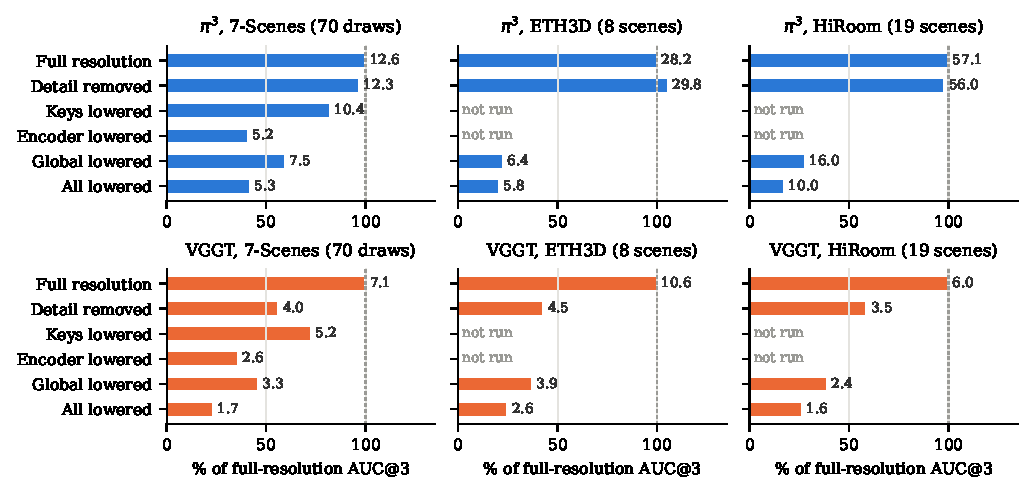
\includegraphics[width=\textwidth]{figures/fig_stages.pdf}
  \caption{\textbf{Every stage we probed needs resolution.} Each bar is the \auc of one probe (\cref{tab:probes}) as a share of the full-resolution input on the same frames; the number beside it is the \auc itself. For \pithree, removing fine pixel detail costs nothing, while lowering the encoder or global attention costs about as much as lowering everything. VGGT loses accuracy under every probe, including removing detail. The encoder and key probes were run on 7-Scenes only.}
  \label{fig:stages}
\end{figure*}

\begin{table}[t]
\centering\small
\setlength{\tabcolsep}{4pt}
\begin{adjustbox}{max width=\linewidth}
\begin{tabular}{@{}lcccc@{}}
\toprule
 & \multicolumn{2}{c}{\pithree} & \multicolumn{2}{c}{VGGT} \\
\cmidrule(lr){2-3}\cmidrule(l){4-5}
Probe (8 of 12 views) & \auc & \aucc & \auc & \aucc \\
\midrule
Full resolution             & 12.6 & 81.9 & 7.1 & 77.8 \\
Detail removed              & 12.3 & 81.4 & 4.0 & 69.7 \\
Encoder lowered             & 5.2  & 70.4 & 2.6 & 66.4 \\
Keys lowered                & 10.4 & 77.4 & 5.2 & 74.5 \\
Global lowered              & 7.5  & 73.0 & 3.3 & 68.5 \\
All lowered                 & 5.3  & 74.5 & 1.7 & 63.2 \\
All lowered, positions not mapped & 1.4 & 51.2 & 0.5 & 31.1 \\
\bottomrule
\end{tabular}
\end{adjustbox}
\caption{\textbf{Stage probes on 7-Scenes} (70 scene-draws). Each row lowers the resolution of the listed stages for 8 of the 12 views (\cref{tab:probes}). Absolute \auc on this dataset is limited by its ground truth (\cref{sec:floor}); \aucc is not.}
\label{tab:stages}
\end{table}

\begin{table}[t]
\centering\small
\setlength{\tabcolsep}{4pt}
\begin{adjustbox}{max width=\linewidth}
\begin{tabular}{@{}lcccc@{}}
\toprule
 & \multicolumn{2}{c}{ETH3D (8 scenes)} & \multicolumn{2}{c}{HiRoom (19 scenes)} \\
\cmidrule(lr){2-3}\cmidrule(l){4-5}
Probe (8 of 12 views) & \pithree & VGGT & \pithree & VGGT \\
\midrule
Full resolution        & 28.2 & 10.6 & 57.1 & 6.0 \\
Detail removed         & 29.8 & 4.5  & 56.0 & 3.5 \\
Global lowered         & 6.4  & 3.9  & 16.0 & 2.4 \\
All lowered            & 5.8  & 2.6  & 10.0 & 1.6 \\
All lowered, not mapped & 1.0 & 0.5  & 1.3  & 0.5 \\
\bottomrule
\end{tabular}
\end{adjustbox}
\caption{\textbf{Stage probes on ETH3D and HiRoom} (pose \auc). Full resolution here is $294{\times}448$ on ETH3D and $364{\times}364$ on HiRoom, which is below VGGT's best size (\cref{fig:response}).}
\label{tab:stages_acc}
\end{table}

\paragraph{The encoder needs full resolution, even for coarse images.}
\emph{Detail removed} and \emph{Encoder lowered} give the network exactly the same image information: both start from the half-resolution image. They differ only in whether the encoder sees that image upsampled to full size or at its own size. For \pithree the difference is large: 12.3 \auc with the full-size encoder against 5.2 with the half-size one, a loss of 7.1 \ci{-8.5}{-5.7}, with the half-size encoder better in only 2 of 70 scene-draws. That loss is about as large as the one from lowering every stage (12.6 to 5.3). Interpolating the encoder's tokens to the full grid does not make up for running the encoder at half resolution. For VGGT the same comparison costs 1.5 \ci{-2.2}{-0.8}.

\paragraph{Global attention needs full resolution too.}
\emph{Global lowered} keeps the pixels, the encoder and frame attention at full resolution and lowers only global attention, together with the heads' view of these 8 views. For \pithree, this alone costs most of what lowering everything costs: 70\% of that loss on 7-Scenes, 97\% on ETH3D (28.2 to 6.4) and 87\% on HiRoom (57.1 to 16.0). Seen the other way, restoring full resolution in the encoder and frame attention while global attention stays at half resolution recovers only 30\%, 2\% and 13\% of the loss on the three datasets. VGGT shows the same pattern at a smaller scale, recovering 29\%, 16\% and 17\%. Resolution is therefore not consumed at a single stage: both the encoder and global attention need it, and full resolution in one cannot make up for its absence in the other.

Mismatched resolution between stages can even hurt coarse accuracy. On ETH3D, \pithree with only global attention lowered reaches 54.8 \aucc, below the 61.6 it reaches with every stage lowered; on 7-Scenes the two are close (73.0 and 74.5). We do not have an explanation for this.

\paragraph{\pithree does not use fine pixel detail; VGGT does.}
Removing the detail above half resolution, while keeping the input size, does not hurt \pithree: its \auc moves from 12.6 to 12.3 on 7-Scenes, rises slightly on ETH3D (from 28.2 to 29.8, a significant $+1.5$, \ci{0.6}{2.6}) and does not change significantly on HiRoom ($-1.1$, \ci{-3.4}{1.1}). VGGT loses accuracy on all three: 3.1 \auc on 7-Scenes, 6.0 on ETH3D \ci{-10.0}{-2.7} and 2.5 on HiRoom \ci{-4.1}{-0.9}.

\paragraph{Positions on a lower-resolution grid must be mapped.}
When a view's tokens sit on a half-resolution grid, its rotary positions describe a smaller image than the full-resolution views'. Mapping them onto the full grid (\cref{eq:align}) is essential: without it, \pithree with every stage lowered drops from 5.3 to 1.4 \auc on 7-Scenes, from 5.8 to 1.0 on ETH3D (a difference of 4.9, \ci{2.8}{7.1}) and from 10.0 to 1.3 on HiRoom, and VGGT loses 2.1 on ETH3D \ci{0.7}{3.7}.

\subsection{Queries and keys in global attention}
\label{sec:keys}

The stage probes leave global attention among the stages that need resolution. This is unwelcome for efficiency, because global attention is the part of the network whose cost grows with the square of the total number of tokens. In attention, though, each token plays two roles: it asks (its query) and it is looked up (its key and value). The two roles need not need the same resolution, so we lower them separately.

Global attention is the stage where views exchange information, and it is the most expensive stage when there are many views. Pooling only the keys and values of the 8 views, while every full-resolution token keeps its own query, costs \pithree 2.3 \auc \ci{-3.6}{-1.0} and VGGT 2.0 \ci{-3.1}{-1.0} on 7-Scenes (\cref{tab:stages}). Starting from the \emph{Detail removed} input instead gives similar losses: 2.2 for \pithree \ci{-3.6}{-0.8} and 2.7 for VGGT \ci{-3.5}{-2.1}. Pooling the queries as well (\emph{Global lowered}) roughly doubles the loss, to 5.1 and 3.9 \auc. For \pithree, pooling keys reduces the transformer compute of these runs by 13\% and pooling queries and keys by 30\%, as estimated from token counts. Queries therefore need full resolution more than keys do, but at 12 views even pooling the keys is not free.

The logit bias that lets a pooled key stand in for the tokens it replaces matters little. Removing it when the encoder is also lowered changes \pithree's \auc by $+0.03$, and adding a similar bias to every lowered view of the \emph{All lowered} probe changes \pithree by $+0.02$ \ci{-0.50}{0.53} and VGGT by $+0.78$ \ci{0.51}{1.06}. How much attention the lowered views receive is thus not the main problem.

\subsection{Errors at different input sizes are correlated}
\label{sec:ensemble}

Every reduction we tried so far costs accuracy, and so does every input size other than a model's best. A remaining hope is that the errors made at different sizes are partly independent, in which case predictions made at several cheap sizes could be combined into one better prediction. We test this on the 70 7-Scenes scene-draws with five uniform input sizes, from $224{\times}294$ to $322{\times}420$. For each pair and triple of sizes, we align the predicted camera sets with a similarity transform, average rotations on SO(3) and camera centres in space, and score the fused poses. Before scoring, we fixed one pair as the test of the idea: the 5{,}184- and 7{,}056-token inputs ($252{\times}336$ and $294{\times}392$). For \pithree, this pair reaches 13.7 \auc, below the 14.4 of the $294{\times}392$ input alone \ci{-1.0}{-0.3}, although it costs more. Across all 20 combinations, every ensemble is significantly worse than the best single size that costs no more, for both models. Only one \pithree ensemble exceeds both of its own members, by 0.3 \auc (12.9 against 12.7 and 12.6). Averaging out a model's error across input sizes therefore does not work, which suggests that most of the error is shared across sizes rather than specific to one.

\subsection{How precise is the benchmark?}
\label{sec:floor}

Throughout these experiments, one dataset behaved differently from the others. Absolute \auc values on 7-Scenes are low for both models (\cref{tab:stages}), and \pithree's response on 7-Scenes is irregular: at uniform sizes from $224{\times}294$ to $322{\times}420$ it scores 9.4, 12.7, 11.7, 14.4 and 12.6, whereas on ETH3D and HiRoom its curve is smooth (\cref{fig:response}). This made us ask how precisely 7-Scenes can measure pose.

We estimated the relative rotation of every pair of views independently, with classical two-view geometry on the full-resolution images: SIFT features, mutual nearest-neighbour matching, and an essential matrix estimated with RANSAC using the dataset's intrinsics. On about 350 pairs with at least 100 inlier matches, the median rotation error against the ground truth is 2.0\textdegree, and only 4\% of these pairs are within 1\textdegree. Changing the assumed focal length from 500 to 620\,px moves this median only between 1.9\textdegree{} and 2.2\textdegree. On the same pairs, \pithree's median error is 1.6\textdegree{} and VGGT's is 1.9\textdegree. Three very different estimators, one of them classical, agree with the ground truth to about the same degree, which points to a limit of the ground truth or its calibration rather than of the methods. We did not establish its cause. Consistent with it, using the classical pair estimates to refine \pithree's poses lowers its \auc on this dataset from 9.4 to 7.9 \ci{-2.3}{-0.7}.

This limit matters for any comparison that relies on \auc on 7-Scenes, since a threshold of 3\textdegree{} is close to the ground truth's own error. We therefore base our response curves on ETH3D and HiRoom, report \aucc alongside \auc, and check the stage findings on all three datasets.

\section{Discussion}
\label{sec:discussion}

\paragraph{What the findings imply.}
Our results suggest four practical consequences. First, a feed-forward 3D model should be evaluated, and compared with others, across a range of input sizes or at its own best size; a single shared size can change a comparison between VGGT and \pithree by almost a factor of ten. Second, more pixels are not automatically better: VGGT degrades above its preferred size, and \pithree stops improving at a size that depends on the data, so larger inputs can add cost without adding accuracy. Third, methods that save compute inside these models should keep the image encoder and the queries of global attention at full resolution; reducing the keys and values of global attention costs less, though at 12 views it is not free. Fourth, fine pose comparisons need ground truth that is more precise than the threshold being measured, which 7-Scenes is not at 3\textdegree.

\paragraph{Why do the models differ?}
VGGT's narrow optimum is consistent with a model that has learned to work at one input size, and \pithree's plateau with one that tolerates a range of sizes. We did not examine the models' training procedures, and we do not establish the cause. Training with a range of input sizes would be the natural way to test it.

\paragraph{Limitations.}
We study two models; Depth Anything~3 and other recent models are not included. All results are exploratory: on ETH3D and HiRoom each scene has one draw of frames, with 8 and 19 scenes, and only 7-Scenes has repeated draws (70 scene-draws). Our probes lower resolution by a factor of 2 per side, for 8 of 12 views, while 4 views stay at full resolution, so they describe how a stage copes with lower resolution in part of the input, not a fully low-resolution stage. One probe lowers global attention and the heads' view of the probed views together, so it does not separate the two. We measure pose only, not reconstruction. We report bootstrap intervals for the comparisons for which we computed them and means otherwise. Our pose metric integrates the exact error distribution, so absolute values differ from those of other evaluation code.

\paragraph{Conclusion.}
We probed how VGGT and \pithree use input resolution. Their responses to resolution have opposite shapes: VGGT works well only near its default input size, while \pithree improves and then levels off. Inside the network, resolution is needed by both the image encoder and global attention, and in global attention more by the queries than by the keys. Their errors at different input sizes are largely shared, and on 7-Scenes the ground truth itself limits how precisely such effects can be measured. We hope these findings help choose input sizes, compare models fairly, and decide where compute can be saved.

{
  \small
  \bibliographystyle{ieeenat_fullname}
  \bibliography{main}
}
\end{document}
